\documentclass[dvipdfmx,autodetect-engine,titlepage]{jsarticle}
\usepackage[dvipdfm]{graphicx}
\usepackage{ascmac}
\usepackage{fancybox}
\usepackage{listings}
\usepackage{plistings}
\usepackage{itembkbx}
\usepackage{amsmath}
\usepackage{svg}
\usepackage{url}
\usepackage{graphics}
\usepackage{listings,jvlisting}

\textheight=23cm
\renewcommand{\figurename}{図}
\renewcommand{\tablename}{表}
\newenvironment{code}
{\vspace{0.5zw}\VerbatimEnvironment  
\begin{screen} 
\baselineskip=1.0\normalbaselineskip
 \begin{Verbatim}}
{\end{Verbatim}
\baselineskip=\normalbaselineskip
 \end{screen}\vspace{0.5zw}} 

\title{情報理工学部 SNコース 3回\\
自然言語処理第5回講義レポート\\}
\author{2600200443-6\\Yamashita Kyohei\\山下 恭平}
\date{May 13 2022}

\begin{document}

\maketitle

\section{解答}

「頭痛を飲み薬でなおした」に形態素解析を行い、得られたラティスは以下の
ものである。

\begin{figure}[h]
  \centering
  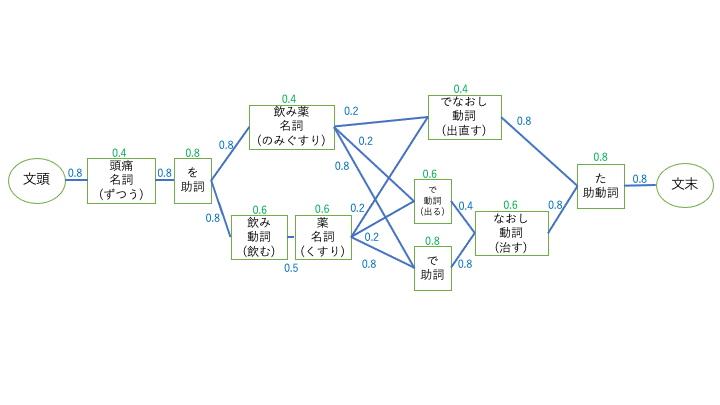
\includegraphics[scale=0.4]{pic1.png}
  \caption{解析結果}
\end{figure}

得られた結果に対して、ヴィタビ・アルゴリズムを用いて制約処理を行ったところ
、最小の累積コストは0.00043487となり、以下のようなラティスが得られた。

\begin{figure}[h]
  \centering
  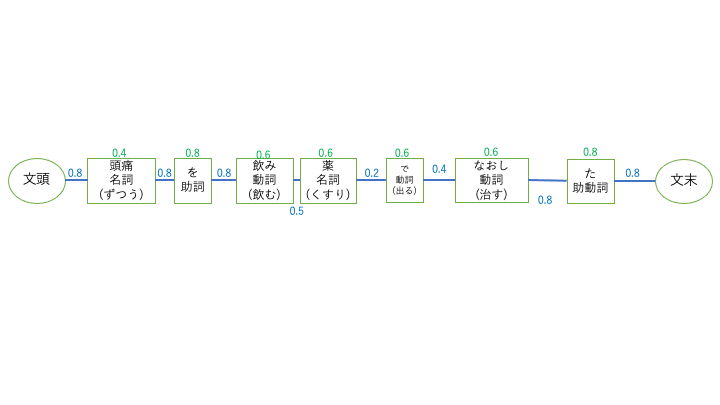
\includegraphics[scale=0.4]{pic21.png}
  \caption{解析結果}
\end{figure}

\end{document}

